\subsection*{Kademlia}

O Kademlia é um \gls*{dht} criado em 2002 \cite{artigo:kademlia} com o objetivo de
melhorar os métodos de busca atuais (Napster e \gls*{gnutella}), que eram ineficientes.
Assim como os outros algoritmos de \gls*{dht}, ele se baseou na estrutura informalmente
conhecida como \enquote{rede de Plaxton} (\emph{Plaxton mesh}), nome que remete a um
dos seus autores \cite{artigo:dht}. Por ter mostrado bons resultados, foi usado na
implementação da busca de arquivos no programa cliente eMule.

A sua modelagem computacional monta um mapa no formato de \gls*{hashtable} onde IDs de
\glspl*{peer} ou de \glspl*{torrent} são chaves para listas de outros \glspl*{peer}.

\subsubsection*{Estrutura de dados}
%\subsubsection*{Tabela de roteamento} ???

O algoritmo implementa uma rede \emph{overlay} cuja estrutura e comunicação se baseiam
na procura de seus nós. Cada um destes nós é identificado por um identificador único
(ID), que serve tanto para a identificação quanto para a localização de valores na
\gls*{hashtable}.

Essa \gls*{hashtable} é na forma de uma árvore binária, cujas folhas são os nós da rede.
Cada folha tem suas posições estabelecidas pelo menor prefixo comum de seus IDs,
organizando-os de forma que, para um dado nó $x$, a árvore é dividida em várias
subárvores menores que não o contém. Assim, a maior subárvore consiste de metade da
árvore que não contém $x$, a subárvore seguinte é feita da metade da árvore restante
onde $x$ também não está contido, etc. O Kademlia garante ainda que todo nó conhece um
outro que está em cada uma das subárvores, se estas contiverem algum nó.

\begin{figure}[ht!]
    \centering
    \fbox{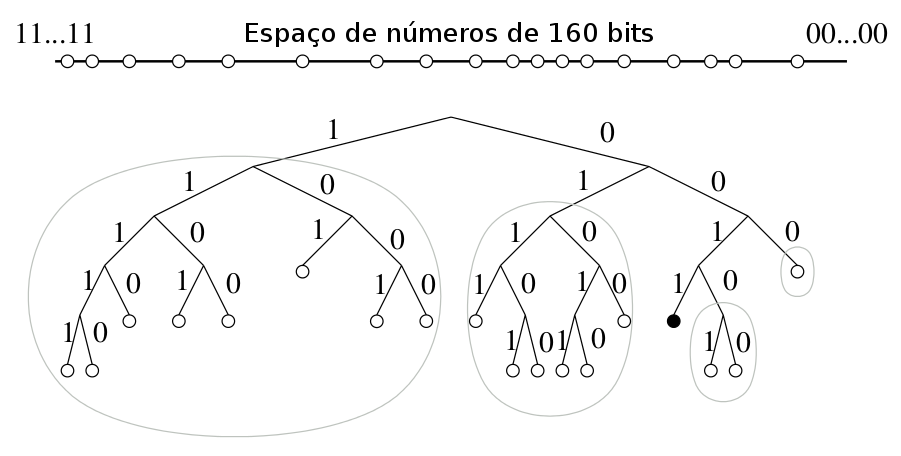
\includegraphics[width=\textwidth]{dht1.png}}
    \caption{Árvore binária do Kademlia. O nó preto é a posição do ID 0011...; os ovais
    cinzas são as subárvores onde o nó preto deve possuir nós conhecidos. Fonte:
    \cite{artigo:kademlia}}
    \label{fig:dht-arvore}
\end{figure}

No Kademlia, objetos e nós possuem IDs únicos de 160 bits: enquanto o primeiro utiliza
o \gls*{hashvalue} de 20 bytes SHA-1 da chave \bverb|info_hash| do \gls*{torrentfile},
o segundo é um valor aleatório escolhido pelo próprio programa.

Durante uma busca por \glspl*{peer} de um \gls*{torrent}, o processo deve conhecer a
chave associado ao objeto, ou seja, o ID, e explora a rede em passos. A cada passo,
encontra nós mais próximos da chave, até chegar ou ao valor buscado ou não nós
existirem mais próximos que o atual. Dessa forma, para uma rede com $n$ nós, o
algoritmo visita apenas $O(\log n)$ nós.

\begin{figure}[ht!]
    \centering
    \fbox{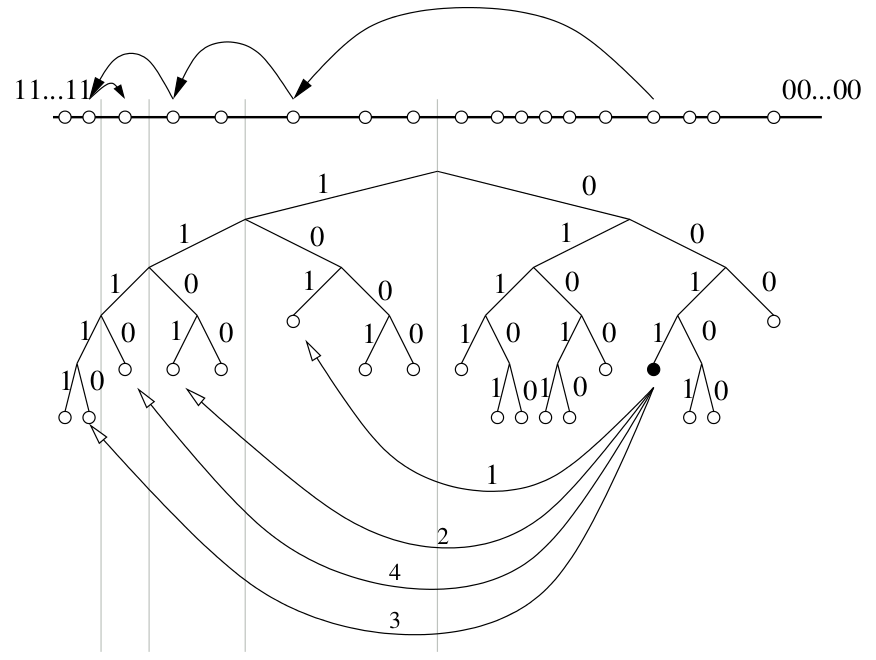
\includegraphics[width=\textwidth]{dht2.png}}
    \caption{Exemplo de uma busca na árvore de nós do Kademlia usando-se um ID. O nó
    preto, de prefixo 0011, encontra o nó de prefixo 1110 através de sucessivas buscas
    (setas numeradas inferiores). As setas superiores mostram a convergência da
    busca durante a execução. Fonte: \cite{artigo:kademlia}}
    \label{fig:dht-arvore-busca}
\end{figure}

Para o conceito de proximidade, as distâncias são calculadas usando-se a função de
distância

\begin{equation}
    d(x,y) = x \oplus y
\end{equation}

que possui algumas propriedades em comum com a equação de distância euclidiana usual,
como as seguintes:

\begin{itemize}
    \item $d(x,x) = 0$
    \item $x \neq y$, $d(x,y) > 0$
    \item simetria: $\forall x,y$, $d(x,y) = d(y,x)$
    \item desigualdade triangular: $d(x,y) + d(y,z) \geq d(x,z)$. \\
        Isto vem do fato de $d(x,z) = d(x,y) \oplus d(y,z)$ e que $\forall a \geq 0,
        \forall b \geq 0 : a + b \geq a \oplus b$
    \item unidirecionalidade: para um dado ponto $x$ e uma distância $\Delta > 0$,
        existe exatamente um ponto $y$ tal que $d(x,y) = \Delta$. Isso garante que todas
        as procuras por uma mesma chave convirjam para um mesmo percurso, independente
        do ponto de partida.
\end{itemize}

\subsubsection*{Tabela de roteamento}

Cada nó do Kademlia armazena informações sobre outros nós para rotear mensagens de
pesquisa. Para cada bit $i$ dos IDs (cada ID tem 160 bits) é mantido um \gls{kbucket},
que contém os nós cuja distância até ele está entre $2^i$ e $2^{i+1}$. Esses
\glspl*{kbucket} são listas de endereço IP, porta de comunicação \gls*{udp} e ID de
nós, ordenadas pelo horário da última notícia destes. Para distâncias pequenas, essas
listas geralmente serão vazias, enquanto para distâncias maiores poderão ser de tamanho
$k$. Este valor, que é o de replicação do sistema, é escolhido de tal forma que esses
$k$ nós possuam grande probabilidade de não falharem na próxima hora.

Quando um nó \textbf{A} recebe uma mensagem de outro nó \textbf{B}, o \gls*{bucket}
correspondente ao ID do remetente (nó \textbf{B}) é atualizado. Disto, podem ocorrer as
seguintes situações:

\begin{itemize}
    \item \textbf{B} já existe no \gls*{bucket}: passa a ser o primeiro da lista, pois
        existiu mensagem recente.

    \item \textbf{B} não existe no \gls*{bucket}:
        \begin{itemize}
            \item \gls*{bucket} não está cheio: \textbf{B} é adicionado no começo da
                lista.
            \item \gls*{bucket} cheio: é enviado um \emph{ping} para o nó do final da
                lista (nó \textbf{C}), contatado há mais tempo

            \begin{itemize}
                \item \textbf{C} não responde ao \emph{ping}: \textbf{C} é retirado da
                lista e \textbf{B} é inserido no início
                \item \textbf{C} responde ao \emph{ping}: \textbf{C} é movido para o
                início da lista e \textbf{B} é ignorado
            \end{itemize}
        \end{itemize}

\end{itemize}

Por conta disso, ocorre que nós mais antigos e funcionais são preferidos, pois quanto
mais tempo um nó está conectado, mais provável ele se manterá conectado por mais 1 hora
\cite{artigo:gnutella-uptime}. Outra vantagem disso é a resistência a alguns ataques de
negação de serviço, pois mesmo que ocorra uma inundação de novos nós, estes só seriam
inseridos nos \glspl*{kbucket} se os antigos fossem excluídos.

\subsubsection*{Funcionamento}

\subsubsubsection{Localizando nós}

\subsubsubsection{Localizando recursos}

\subsubsubsection{Entrando na rede}

\subsubsubsection{Saindo da rede}